\documentclass[conference]{IEEEtran}
\IEEEoverridecommandlockouts
% The preceding line is only needed to identify funding in the first footnote. If that is unneeded, please comment it out.
\usepackage{cite}
\usepackage{amsmath,amssymb,amsfonts}
\usepackage{algorithmic}
\usepackage{graphicx}
\usepackage{textcomp}
\usepackage{dsfont}
\usepackage{xcolor}
\usepackage[utf8]{inputenc}
\usepackage{url}
\usepackage[export]{adjustbox}
\def\BibTeX{{\rm B\kern-.05em{\sc i\kern-.025em b}\kern-.08em
    T\kern-.1667em\lower.7ex\hbox{E}\kern-.125emX}}
\begin{document}

\title{Text Classification for Twitter Sentiment\\
}

\author{\IEEEauthorblockN{1\textsuperscript{st} Igor Mourão Ribeiro}
\IEEEauthorblockA{\textit{Computer Engineering Departament} \\
\textit{Instituto Tecnológico de Aeronáutica}\\
São José dos Campos, Brazil \\
igormr98mr@gmail.com}
\and
\IEEEauthorblockN{2\textsuperscript{nd} Isabelle Ferreira de Oliveira}
\IEEEauthorblockA{\textit{Computer Engineering Departament} \\
\textit{Instituto Tecnológico de Aeronáutica}\\
São José dos Campos, Brazil \\
isabelle.ferreira3000@gmail.com}
\and
\IEEEauthorblockN{3\textsuperscript{rd} José Luciano de Morais Neto}
\IEEEauthorblockA{\textit{Computer Engineering Departament} \\
\textit{Instituto Tecnológico de Aeronáutica}\\
São José dos Campos, Brazil \\
zluciano.t19@gmail.com}
%\and
%\IEEEauthorblockN{4\textsuperscript{th} Thiago Filipe de Medeiros}
%\IEEEauthorblockA{\textit{Computer Engineering Departament} \\
%\textit{Instituto Tecnológico de Aeronáutica}\\
%São José dos Campos, Brazil \\
%thiagoofic@gmail.com}
}

\maketitle


\begin{abstract}
Esse relatório documenta a implementação de algoritmos de Processamento de Linguagem Natural, aplicando diferentes técnicas de Machine Learning para classificar Tweets entre sentimentos positivos e negativos. Os algoritmos implementados foram Naive Bayes e Support Vector Machine, utilizando diferentes features produzidas a partir de um dataset do Kaggle, e comparando-os pelas métricas de acurácia e coeficiente Kappa.
\end{abstract}

\begin{IEEEkeywords}
Processamento de Linguagem Natural, Naive Bayes, Aprendizagem Supervisionada, Support Vector Machine
\end{IEEEkeywords}

\section{Introdução}
Um dos aspectos relevantes da interação entre as pessoas na atualidade é a expressão de sentimentos por meio de textos nas mídias sociais. Nesse contexto, o monitoramento das redes sociais pode ser explorado como forma de extrair a aceitação e/ou aprovação de produtos e também obter conhecimento dos usuários. A análise de sentimentos surge da necessidade de tratar e interpretar textos, opiniões e comentários realizados pelos usuários em redes sociais. Por meio das informações subjetivas extraídas textos em linguagem natural, pode ser gerado conhecimento estruturado, auxiliando a tomada de decisão. 

A expansão da Internet e a utilização das redes sociais definiram um ecossistema de interação, no qual os usuários deixaram de ser receptores passivos e se tornaram produtores, compartilhadores e avaliadores de conteúdo. Em um cenário onde as reputações de empresas e a aceitabilidade de produtos no mercado são diretamente afetadas pela repercussão de opiniões de seus clientes na web, tanto quanto pelas campanhas de publicidade, a análise de sentimentos surge como um diferencial para rastreamento do conteúdo emocional daquilo que se escreve e compartilha nas redes sociais. Nesse sentido, a análise de sentimentos alia-se à publicidade promovendo subsídios para definição de estratégias e garantia da vantagem competitiva.

A análise de sentimentos ser aplicada na gestão de informação por exemplo, fornecendo feedback do cliente a partir do conteúdo dos diversos canais de comunicação e entregando informações úteis para tomada de decisão e definição de estratégias para satisfação dos clientes.

O Twitter\cite{twitter} é uma rede social e servidor para microblogging muito utilizada, que será utilizada para essa análise de sentimentos. Atualmente, o limite máximo de um \textit{tweet} (mensagem postada no blog) é de 280 caracteres e tem-se um total de 6000 \textit{tweets} por segundo o que implica em 200 bilhões por ano. Exemplos de \textit{tweets} com emoções podem ser vistos nas Figuras \ref{fig:dataset_positivo} e \ref{fig:dataset_negativo}.

\begin{figure}[htbp]
	
\includegraphics[width=0.5\textwidth,center]{imgs/tweet_positivo.png}
	\caption{\textit{Tweet} com mensagem positiva}
	\label{fig:dataset_positivo}
\end{figure}


\begin{figure}[htbp]
	
\includegraphics[width=0.5\textwidth,center]{imgs/tweet_negativo.png}
	\caption{\textit{Tweet} com mensagem negativa}
	\label{fig:dataset_negativo}
\end{figure}

Neste sentido, este trabalho tem como objetivo apresentar a análise de
sentimentos aplicada a textos em linguagem natural de uma rede social, usando diversos modelos e entradas para posterior comparação.

\section{Fundamentos Teóricos}

\subsection{Definições}

Neste projeto, são utilizadas as notações $m_i$, para a $i$-ésima mensagem em uma amostra do \textit{dataset} com $1 \leq i \leq M$ (sendo $M$ o número de mensagens na amostra) e correspondendo a um vetor frequência de \textit{features} $f(x_{j}, m_i)$, onde $x_{j}$ representa a $j$-ésima \textit{feature} da mensagem $m_i$. Cada vetor $m_i$ de frequência de \textit{features} tem a mesma dimensão $F$, correspondendo à quantidade de \textit{features} consideradas, i. e., $1 \leq j \leq F$.

As \textit{features} são a menor unidade de informação considerada em uma mensagem. Foram consideradas quatro tipos de \textit{features}: \textit{Count Vectors} (CV), Palavra à palavra, Caracter à caracter e $N$-Grams. No caso das três últimas \textit{features} referidas, foi considerado o modelo \textit{Term-Frequency Inverse Document Frequency}, enquanto a \textit{feature} CV seguiu o modelo \textit{Term Frequency}, ambos apresentados na seção $D$.

\subsection{Naive-Bayes}

Considerando as classes $C_k$ a serem classificadas as mensagens $m$ (no caso deste projeto $C_1 = \text{positiva}$ e $C_2 = \text{negativa}$), o modelo \textit{Naive-Bayes} realiza a classificação por meio da maximização da probabilidade $P(C_k | m)$, ou seja, busca a classe $k$ que maximiza tal probabilidade. Para tanto, o \textit{teorema de Bayes}, apresentado na \textbf{Equação \eqref{eq:bayes}}, é utilizado

\begin{equation} \label{eq:bayes}
P(C_k | m) = \frac{P(C_k) P(m | C_k)}{P(m)}
\end{equation}

\noindent a suposição do modelo (e que dá nome ao mesmo) é que as \textit{features} $x_{j}^m$ em uma mensagem $m$ são independentes. Assim, a probabilidade condicional $P(m | C_k)$ toma a forma apresentada na \textbf{Equação \eqref{eq:ind_prob_cond}},

\begin{equation} \label{eq:ind_prob_cond}
P(m | C_k) = \prod_{j=1}^F P(x_{j}^m | C_k)^{f(x_j, m)}
\end{equation}

\noindent na qual $f(x_j, m)$ é a frequência de ocorrência da \textit{feature} $x_j$ na mensagem $m$ (definida na seção $D$), e de onde podemos expressar a probabilidade $P(C_k | m)$ como na \textbf{Equação \eqref{eq:naive_bayes}},

\begin{equation} \label{eq:naive_bayes}
P(C_k | m) = \alpha P(C_k) \prod_{j=1}^F P(x_{j}^m | C_k)^{f(x_j, m)}
\end{equation}

\noindent onde a constante de normalização $\alpha$ independe das classes $C_k$ \cite{kibriya}. Enfim, o modelo realiza a classificação por meio da estimativa $\hat{C}_m$, dada pela \textbf{Equação \eqref{eq:naive_bayes_estimation}},

\begin{equation} \label{eq:naive_bayes_estimation}
\hat{C}_m = \underset{k} {argmax}\left\{P(C_k | m)\right\}
\end{equation}

\indent As probabilidades $P(x_{j}^m | C_k)$ são estimadas em conjunto com a \textit{suavização de Laplace}, por meio da \textbf{Equação \eqref{eq:estimator}},

\begin{equation} \label{eq:estimator}
\hat{P}(x_{j}^m | C_k) = \frac{1 + \sum\limits_{m_p \in C_k} f\left(x_{j},m_p \right)}{F + \sum\limits_{q | m_r \in C_k} f\left(x_{q}, m_r\right)}
\end{equation}

\noindent onde a soma no numerador se dá sobre todas as mensagems $m_p$ da amostra do \textit{dataset} que pertencem à classe $C_k$  e a soma no denominador se dá sobre todas as \textit{features} $x_{q}$ de todas as mensagems $m_r$ da amostra do \textit{dataset} que pertencem à classe $C_k$. As probabilidades $P(C_k)$ são estimadas pela simples frequência das classes na amostra do \textit{dataset}, ou seja,

\begin{equation} \label{eq:class_prob}
\hat{P}(C_k) = \frac{\sum\limits_p \mathds{1}\left[m_p \in C_k\right]}{M}
\end{equation}

\noindent onde o somatório no numerador conta a quantidade de mensagens classificadas como pertencentes à classe $C_k$. 

\subsection{Support Vector Machine - (SVM)} 

A ideia principal de uma SVM \cite{svm} é a de dividir o dataset através de um hiperplano que separe os dados nas duas classificações previstas no seu rótulo de acordo com o apredizado supervisionado.

Além disso, uma margem é definida a partir desse hiperplano que separa as classificações e as distancia uma da outra, como pode ser visot na ilustrção a seguir:

\begin{figure}[htbp]
	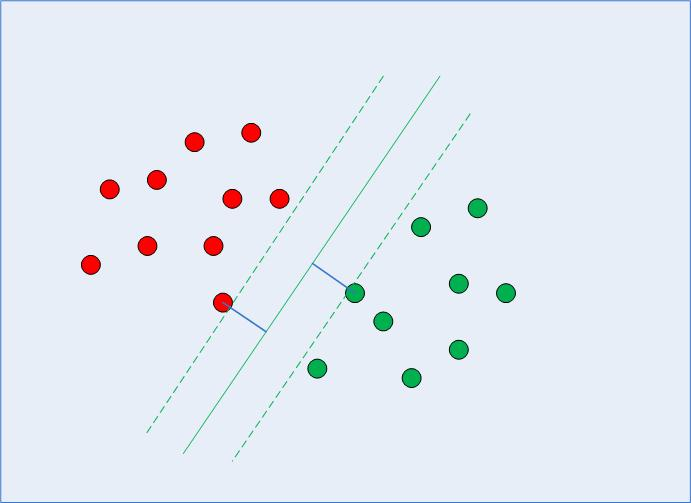
\includegraphics[width=0.4\textwidth,center]{imgs/svm.jpg}
	\caption{Exemplo ilustrativo de uma divisão feita por um SVM.}
	\label{fig:svm_exemple}
\end{figure}

A escolha do hiperplano e da margem, i.e. os parâmetros escolhidos para se definir a separação do \textit{dataset}, é feita de tal forma que o erro associado às más classificações de dados presentes no \textit{dataset} de treinamento seja minimizado.

A escolha é feita dessa forma para que o risco associado seja mínimo. Entende-se por risco, a probabilidade de se errar uma futura classificação de um dado desconhecido.

\subsection{Term Frequency - Inverse Document Frequency}

A princípio, as frequências $f\left(x_j, m_p\right)$ da seção $B$ poderiam ser calculadas como a quantidade de vezes que a \textit{feature} $x_j$ está presente nas mensagens $m_p$. Esta é a chamada \textit{Term Frequency} (TF), apresentada nas \textbf{Equações \eqref{eq:term_frequency} e \eqref{eq:norm_term_frequency}},

\begin{equation} \label{eq:term_frequency}
f_{TF}(x_{j}, m_p) = \sum_{w \in m_p} \mathds{1}\left[w = x_{j}\right]
\end{equation}

\begin{equation} \label{eq:norm_term_frequency}
f_{nTF}(x_{j}, m_p) = \frac{f_{TF}(x_j, m_p)}{\sum\limits_q f_{TF}(x_q, m_p)}
\end{equation}

\noindent onde o somatório na \textbf{Equação \eqref{eq:term_frequency}} se dá sobre todos os termos presentes na mensagem $m_p$ e a \textbf{Equação \eqref{eq:norm_term_frequency}} representa a \textit{Term Frequency} normalizada pela quantidade de termos na mensagem $m_p$. Porém, uma outra representação, chamada \textit{Term Frequency - Inverse Document Frequency} (TF-IDF), se mostrou mais eficaz na classificação de texto em documentos (no caso deste projeto, mensagems). A $f_{TFIDF}$ é dada pelas \textbf{Equações} \eqref{eq:tf_idf} e \eqref{eq:idf},

\begin{equation} \label{eq:tf_idf}
f_{TFIDF}(x_j, m_p) = f_{nTF}(x_j, m_p) \cdot f_{IDF}(x_j)
\end{equation}

\begin{equation} \label{eq:idf}
f_{IDF}(x_j) = log\left(\frac{M}{\sum\limits_{q} \mathds{1}\left[f_{TF}(x_j, m_q) \neq 0\right]}\right)
\end{equation}

\noindent onde $f_{IDF}(x_j)$ é o \textit{Inverse Document Frequency}, o logaritmo do inverso da fração de mensagens da amostra onde a \textit{feature} $x_j$ ocorre.

\subsection{Coeficiente Kappa de Cohen}

Dependendo dos dados escolhidos, mesmo que ao acaso, para o treinamento das diferentes redes neurais, vários enviesamentos podem acontecer e, por esse motivo, existe uma maneira de comparar duas formas de classificação através do Coeficiente Kappa de Cohen \cite{kappa}.

O objetivo deste coeficiente é de comparar, entre dois tipos de classificação, o grau de acordo a partir da seguinte equação:

\begin{equation} \label{eq:kappa}
\kappa = \frac{P_o - P_e}{1 - P_e}
\end{equation}

Onde $P_o$ representa a proporção de casos em que ambos classificaram na mesma categoria, enquanto que $P_e$ representa a probabilidade da classificação na mesma categoria ocorrer por mera coincidência.

Quão mais próximo de $P_e$ for $P_o$, temos que a proporção de concordância se aproxima da probabilidade de acerto por coincidência, ou seja, a concordância se aproxima do aleatório e o valor de $\kappa$ se aproxima de $0$. Enquanto que quanto mais próximo de $1$ for $P_o$, temos que a concordância se aproxima da concordância absoluta e o valor de $\kappa$ se aproxima de $1$.

Assim, à medida que $\kappa$ varia de $0$ a $1$, a concordância entre as classificações fica cada vez maior.

\section{Proposta}

Neste trabalho, propomos a utilização de classificadores baseados em \textit{Naive-Bayes} e SVMs para a classificação da positividade de \textit{tweets}. Foram experimentadas diversos tipos de \textit{features} a fim de se realizar uma comparação da performance dos classificadores: para o \textit{Naive-Bayes}, foram testados os modelos de \textit{Count Vector} (TF), Palavra à palavra (TF-IDF), $N$-Gram (de palavras com TF-IDF) e Caracter à caracter (também com TF-IDF); para a SVM, foi testado o uso de $N$-Gram (de palavras com TF-IDF).

\section{Metodologia}

O projeto foi implementado na linguagem \textit{Python 3}, fazendo uso da biblioteca \textit{scikit-learn}, feita para aplicações de \textit{Machine Learning}.

Foi utilizado um \textit{dataset} obtido no \textit{website} Kaggle com $1.6$ milhões de \textit{tweets}, todos em inglês, em que, para cada \textit{tweet}, há um número de $0$ a $4$ expressando a positividade do mesmo (4 mais positivo e 0 mais negativo). O \textit{dataset} completo pode ser encontrado em \cite{dataset_completo}.

Inicialmente, foi feito um pré-processamento do \textit{dataset}, de forma a extrair os dados necessários para o treinamento e para retirar caracteres no texto que não são úteis para a classificação.

Foram removidos do \textit{dataset} os campos de data que o \textit{tweet} foi feito e o ID único de cada \textit{tweet}. Com isso, obtiveram-se apenas a classificação da positividade e o texto para cada \textit{tweet}.

Em seguida, foi feito o pré-processamento de texto, em que, inicialmente, foi colocado todo em minúsculo. Além disso, por meio de uma análise qualitativa de \textit{tweets}, foram notados diversos nomes de pessoas marcadas no texto, representadas quando a palavra começa com um '@'. Esses nomes não ajudam na classificação do texto, assim como pontuações e números, de forma que foram eliminadas a presença de quaisquer caracteres não alfabéticos do texto, enquanto eliminado o nome de pessoas referenciados no texto.

Por último, foram randomizadas as entradas do \textit{dataset}, de forma a diminuir o \textit{bias} no treinamento. Depois o \textit{dataset} foi separado em 75\% para o conjunto de treinamento e 25\% para o conjunto de testes. Finalmente, por motivos do treinamento do \textit{dataset} completo não poder ser realizado devido ao limite de memória (8GB de RAM), foram utilizadas apenas $1$ milhão de entradas para o treinamento com o modelo \textit{Naive Bayes} e $100$ mil entradas para o SVM. O número menor de entradas para o SVM é justificado em seu grande custo computacional no treinamento.

\section{Experimentos, Resultados e Análise}

A seguir tem-se duas tabelas que ilustram os resultados obtidos com os experimentos. Na primeira podem ser observados a acurácia dos resultados e dos testes para cada método utilizado de treinamento:

\begin{table}[htbp]

\caption{Porcentagens de acerto dos modelos nos conjuntos de teste e treinamento}
\begin{center}
\begin{tabular}{|c|c|c|c|c|c|} \hline
\textbf{Modelo} & \multicolumn{4}{|c|}{\textbf{\textit{Naive Bayes}}} & \textbf{SVM} \\ \hline
\textbf{\textit{Features}} & \textbf{\textit{CV}}$^{\mathrm{a}}$ &  \textbf{\textit{Word}}$^{\mathrm{b}}$ & \textbf{\textit{N-Gram}$^{\mathrm{b}}$} & \textbf{\textit{Char}$^{\mathrm{b}}$} & \textbf{\textit{N-Gram}$^{\mathrm{b}}$} \\ \hline
\textbf{Treino} & $81.71\%$ & $77.28\%$ & $77.52\%$ & $74.18\%$ & $70.49\%$ \\
\textbf{Testes} & $78.17\%$ & $77.03\%$ & $77.41\%$ & $74.13\%$ & $68.63\%$ \\
\hline
\multicolumn{6}{l}{$^{\mathrm{a}}$ segundo o modelo TF.}\\
\multicolumn{6}{l}{$^{\mathrm{b}}$ segundo o modelo TF-IDF.}
\end{tabular}
\label{tab1}
\end{center}

\end{table}

O cálculo para o valor de Kappa para cada modelo foi feito considerando uma comparação com os próprios rótulos dos dados \cite{cohen_score}, ou seja, a comparação foi feita com um classificador perfeito que tem 100\% de acurácia com o \textit{dataset}. Esses valores podem ser vistos na tabela a seguir:

\begin{table}[htbp]

\caption{Valores do coeficiente kappa para cada modelo}
\begin{center}
\begin{tabular}{|c|c|c|c|c|c|} \hline
\textbf{Modelo} & \multicolumn{4}{|c|}{\textbf{\textit{Naive Bayes}}} & \textbf{SVM}$^{\mathrm{a}}$ \\ \hline
\textbf{\textit{Features}} & \textbf{\textit{CV}$^{\mathrm{a}}$} &  \textbf{\textit{Word}$^{\mathrm{b}}$} & \textbf{\textit{N-Gram}$^{\mathrm{b}}$} & \textbf{\textit{Char}$^{\mathrm{b}}$} & \textbf{\textit{N-Gram}$^{\mathrm{b}}$} \\ \hline
\textbf{Kappa}  & $0.563$ & $0.541$ & $0.584$ & $0.482$ & $0.361$ \\
\hline
% \multicolumn{6}{l}{$^{\mathrm{a}}$\textit{Support Vector Machine} (SVM)}.\\
\multicolumn{6}{l}{$^{\mathrm{a}}$ segundo o modelo TF.}\\
\multicolumn{6}{l}{$^{\mathrm{b}}$ segundo o modelo TF-IDF.}
\end{tabular}
\label{tab2}
\end{center}

\end{table}

Quando um classificador randômico tenta classificar os dados, é esperado que ainda se obtenha uma acurácia de 50\% pois estaria acertando de maneira aleatória. O que importa mesmo é a acurácia da classificação entre 50\% e 100\%, pois é a partir daí que se ressalta o diferencial perante um palpite randômico.

Como era de se esperar, o valor de Kappa reflete exatamente isso. Seu valor variando de $0$ a $1$ representa a acurácia de cada método variando de 50\% a 100\%. Como podemos ver a seguir:

\begin{equation} \label{eq:kappa}
\kappa = \frac{P_1 - P_2}{1 - P_2}
\end{equation}

\noindent $P_1$ representa a concordância do método com o valor do rótulo, ou seja, a acurácia dos testes. $P_2$ representa a probabilidade de acertar o valor de maneira aleatória que, por se tratar de 2 valores possíveis de rótulos e considerando que o \textit{dataset} está bem distribuído, vale em torno de 50\%.

Isso significa que, embora o entedimento estatístico do problema permita fazer essa observação sobre os valores de acurácia que realmente importam, o valor de Kappa dispensa esse conhecimento e dá um valor significativo sobre o quão bom é cada classificador.

\section{Conclusões}

Pode-se concluir através dos resultados que o SVM, mesmo exigindo um processamento muito grande e trabalhando com 10\% do tamanho padronizado de dados, foi o que teve o pior resultado, sendo assim um classificador ruim se comparado aos demais.

Sendo assim, o método de \textit{Naive-Bayes} foi consideravelmente se baseando nos valores de Kappa obtidos. Sendo o método em \textit{Word-Level} ligeiramente melhor que os demais, embora todos, tenham tido um desempenho similar, com exceção do método em \textit{Char-Level} que teve um desempenho um pouco menor entre os que foram feitos baseados em \textit{Bayes}.

\begin{thebibliography}{00}
\bibitem{dataset_completo} Dataset de Sentimentos, \url{https://www.kaggle.com/kazanova/sentiment140}.
\bibitem{twitter} Twitter, \url{https://twitter.com}
\bibitem{kibriya} Kibriya, Ashraf \& Frank, E. \& Pfahringer, Bernhard \& Holmes, Geoffrey. (2004). Multinomial naive Bayes for text categorization revisited. Advances in Artificial Intelligence. 488-499. \label{kibriya}
\bibitem{https://scikit-learn.org/stable} SciKit-Learn, \url{https://scikit-learn.org/stable/}
\bibitem{kappa} Cohen, Jacob (1960). "A coefficient of agreement for nominal scales". Educational and Psychological Measurement. 20 (1): 37–46. \url{doi:10.1177/001316446002000104}
\bibitem{svm} Implementing SVM and Kernel SVM with Python's Scikit-Learn \url{https://stackabuse.com/implementing-svm-and-kernel-svm-with-pythons-scikit-learn/}
\bibitem{cohen_score} sklearn.metrics.cohen\_kappa\_score \url{https://scikit-learn.org/stable/modules/generated/sklearn.metrics.cohen_kappa_score.html}

\end{thebibliography}

\end{document}
